 \documentclass[a4paper,10pt,oneside]{article}
\usepackage[polutonikogreek,italian]{babel}
\usepackage[utf8x]{inputenc}
\usepackage{amsmath}
\usepackage{amsthm}
\usepackage{amssymb}
\usepackage{amscd}
\usepackage{graphicx}
\usepackage{float}
\usepackage{array}
\usepackage{verbatim}
\usepackage{rotating}
\usepackage[small]{caption}
\usepackage{lscape}
\usepackage{fancybox}
\usepackage{booktabs}
\parindent0ex 
\renewcommand{\fboxsep}{0.5cm}
\usepackage{hyperref}
\renewcommand{\textfraction}{0.05}
\renewcommand{\topfraction}{0.95}
\renewcommand{\bottomfraction}{0.95}
\renewcommand{\floatpagefraction}{0.35}
\setcounter{totalnumber}{5}
\restylefloat{figure}
\newlength{\drop}
\begin{document}

\begin{center}
{\huge Laboratorio di  meccanica 2}
\end{center}


\begin{abstract}
Durante questo laboratorio analizzeremo il principio di conservazione della quantità di moto e tramite degli esperimenti cercheremo di vedere come in assenza di forze esterne il momento lineare sia costante \footnote{Momento lineare=Quantità di moto}.
\end{abstract}


\section{Richiami teorici}
Possiamo ricavare la legge di conservazione della quantità di moto in due modi diversi, nel primo ipotizzeremo che le forze in gioco nel sistema siano di tipo newtoniano, ovvero che in ogni istante valga la relazione $F_{12}=-F_{21}$ mentre nel secondo dedurremo la conservazione della quantità di moto da quella dell'energia e dall'invarianza galileiana.
Ricordando che la quantità di moto (nel caso non relativistico) è definita come:
\begin{equation}
 \mathbf{p}=m\mathbf{v}
\end{equation}
possiamo scrivere la prima legge di Newton in forma più generale come:
\begin{equation}
 \mathbf{F}=\frac{d\mathbf{p}}{dt}
\end{equation}
che si riduce alla forma standard della prima legge della meccanica nel caso in cui la massa sia costante.
Per ricavare la legge di conservazione della quantità di moto applichiamo il terzo principio della dinamica a due corpi in interazione (ad esempio due sfere che collidono) per un determinato intervallo di tempo finito $\Delta t$, le forze risultanti saranno:
\begin{equation}
 F_{12}=M_1\frac{\Delta \mathbf{v}_1}{\Delta t}
\end{equation}
e 
\begin{equation}
 F_{21}=M_2\frac{\Delta \mathbf{v}_2}{\Delta t}
\end{equation}
per il terzo principio possiamo scrivere:
\begin{equation}\label{terzo}
 M_1\frac{\Delta \mathbf{v}_1}{\Delta t}=-M_2\frac{\Delta \mathbf{v}_2}{\Delta t}
\end{equation}

La relazione [\ref{terzo}] deve valere per ogni intervallo di tempo $\Delta t$, questo ci permette di scrivere:
\begin{equation}\label{princ}
 (M_1\mathbf{v}_1+M_2\mathbf{v}_2)_{iniziale}=(M_1\mathbf{v}_1+M_2\mathbf{v}_2)_{finale}
\end{equation}

La [\ref{princ}] vale chiaramente solo supponendo che le forze si propaghino con velocità infinita\footnote{Ovvero nell'ipotesi di forze newtoniane}.


\section{Esperienza di laboratorio}

Nella prima esperienza di laboratorio utilizzeremo un piccolo petardo per imprimere una velocità non nulla su due carrelli fluttuanti sopra la guidovia a cuscino d'aria.
\begin{figure}[H]
 \centering
 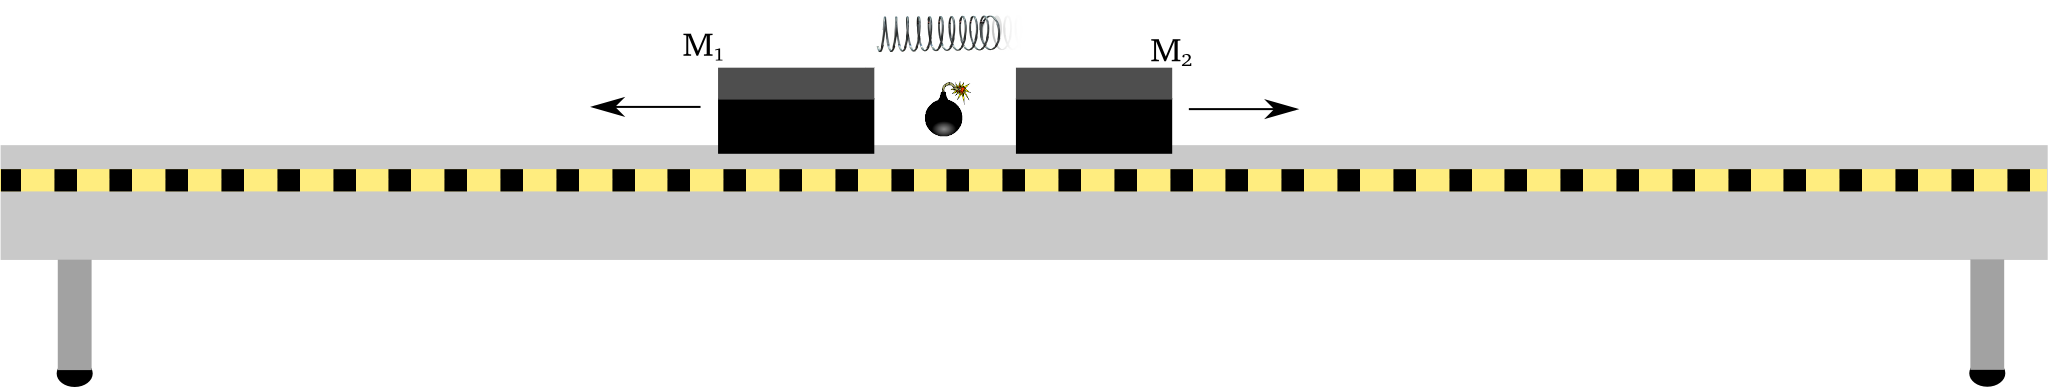
\includegraphics[width=\textwidth]{./Immagini/text5895-9.png}
 % text5895-9.png: 2048x387 pixel, 201dpi, 25.89x4.89 cm, bb=
 \caption{Tramita una molla o un piccolo petardo i carrelli fluttuanti iniziano a muoversi lungo la guidovia}
 \label{fig:esplosione}
\end{figure}

La procedura sperimentale è la seguente:
\begin{itemize}
 \item Mettiamo in stazione la guidovia e ci accertiamo che sia perpendicolare alla direzione della forza di gravità
\item Posizioniamo i carrelli e facciamo aderire la camera di scoppio
\item Posioniamo il petardo e lo accendiamo
\item Simultaneamente all'accensione del petardo iniziamo l'acquisizione dati con il software Pasco
\item Misuriamo per alcuni istanti dopo lo scoppio la variazione di posizione dei carrelli
\end{itemize}

La quantità di moto prima dello scoppio sarà:
\begin{equation}\label{cons_1}
 (M_1+M_2+M_p)\mathbf{v}_i
\end{equation}

per uno stazionamento perfetto di carrelli e guidovia possiamo ottenere $v_i=0$.
La quantità di moto dopo lo scoppio sarà:

\begin{equation}\label{cons_2}
 M_1\mathbf{v}_{f1}+M_2\mathbf{v}_{f2}+\sum_km_k\mathbf{v}_k
\end{equation}

dove $\sum_km_k\mathbf{v}_k$ è la somma delle quantità di moto dei pezzetti in cui si è suddiviso il petardo.


Uguagliando le relazioni [\ref{cons_1}] e [\ref{cons_2}] otteniamo:


\begin{equation}\label{lab_cons}
  (M_1+M_2+M_p)\mathbf{v}_i=M_1\mathbf{v}_{f1}+M_2\mathbf{v}_{f2}+\sum_km_k\mathbf{v}_k
\end{equation}

dopo aver terminato l'acquisizione dati verificheremo che effettivamente (a meno di errori sperimentali) la quantità di moto prima dell'esplosione è uguale alla quantità di moto dopo l'esplosione. La stessa procedura descritta per l'esplosione dovrà essere seguita nel caso in cui la forza interna che mette in moto i carrelli sia quella della molla.
L'ultima parte dell'esperienza sulla conservazione della quantità di moto è la misura della velocità di uscita dell'acqua da una siringa o da una pistola ad acqua. 
\begin{figure}[H]
 \centering
 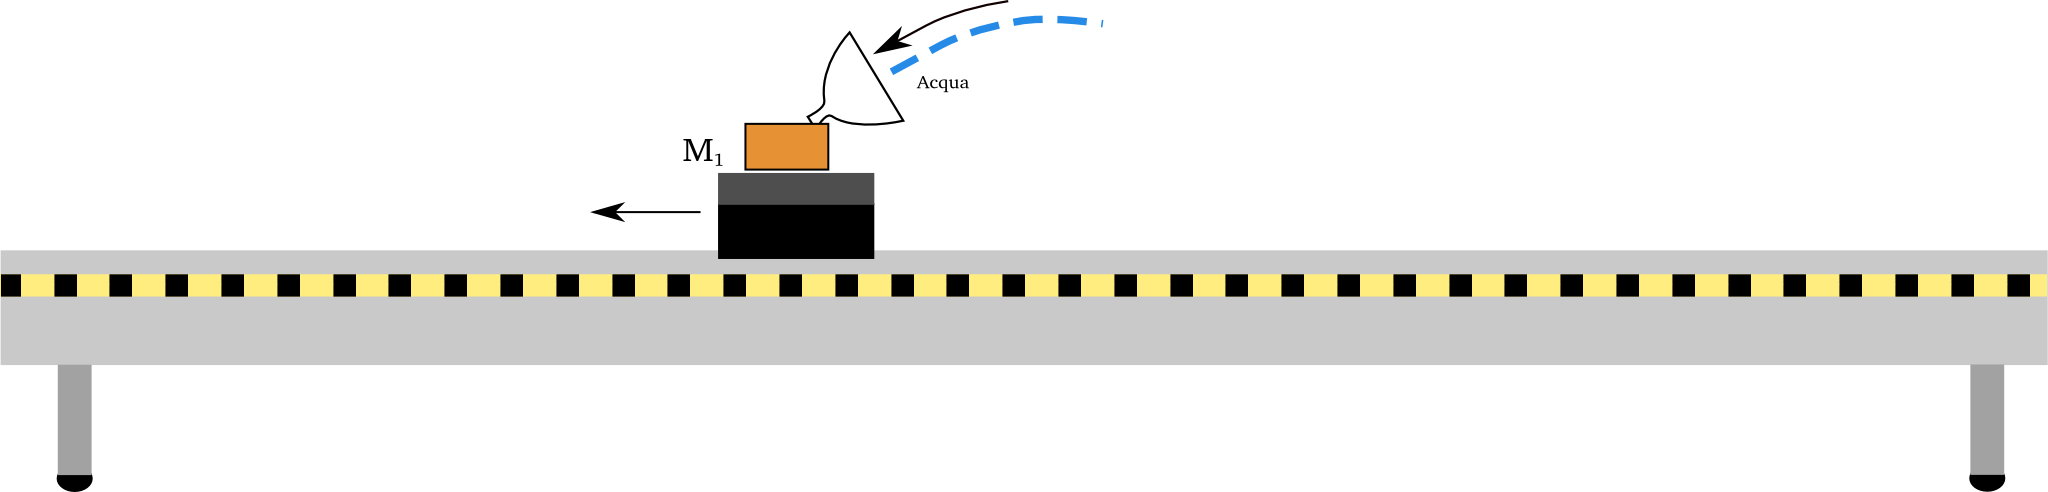
\includegraphics[width=\textwidth]{./Immagini/imbuto.png}
 % imbuto.png: 2048x492 pixel, 201dpi, 25.89x6.22 cm, bb=
 \caption{Tramite una siringa caricata ad acqua trasferiamo della quantità di moto al carrello fluttuante}
 \label{fig:imbuto}
\end{figure}
possiamo scrivere la relazione:
\begin{equation}
 M_c\mathbf{v}_{i_{carrello}}+M_a\mathbf{v}_{i_{ugello}}=(M_c+M_a)\mathbf{v}_f
\end{equation}






\end{document}
